% Created by tikzDevice version 0.12 on 2018-09-20 18:19:13
% !TEX encoding = UTF-8 Unicode
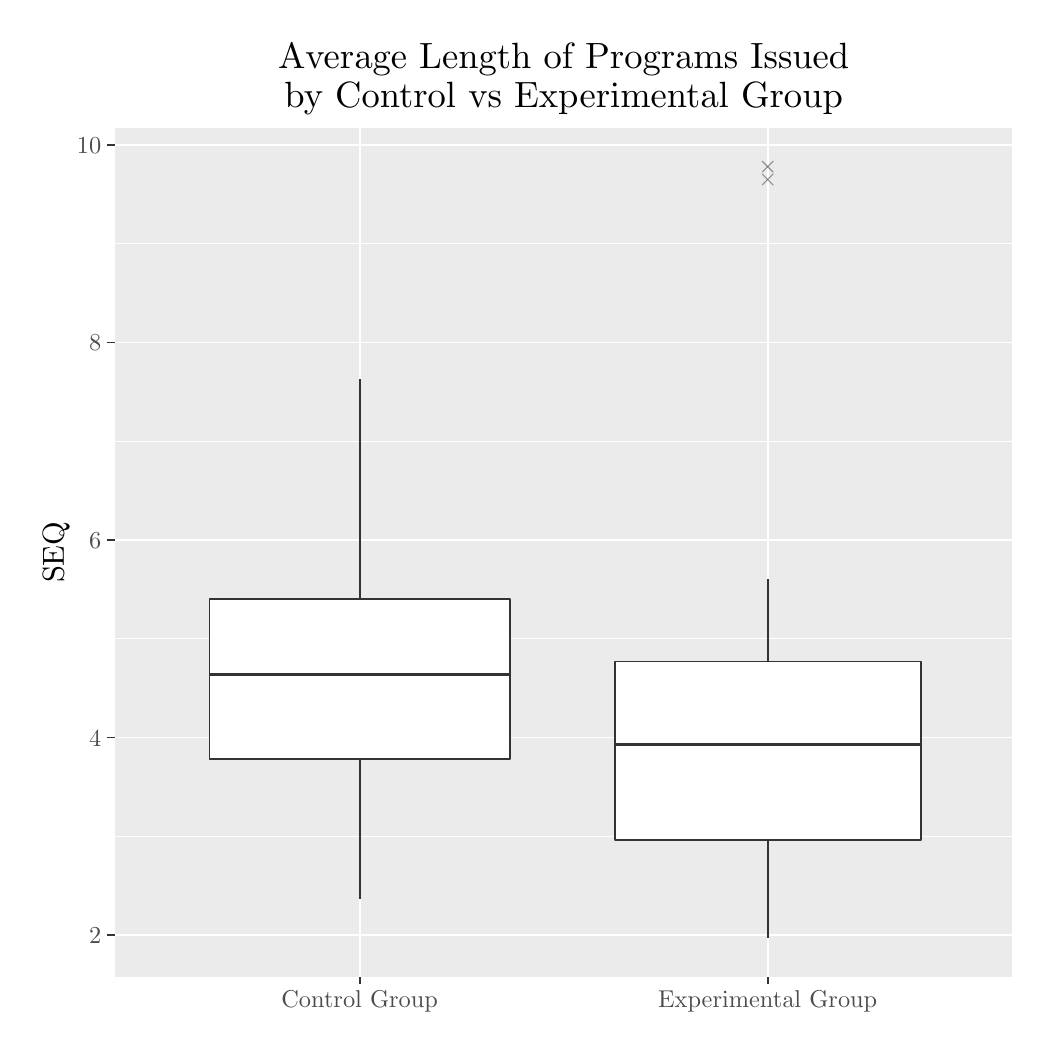
\begin{tikzpicture}[x=1pt,y=1pt]
\definecolor{fillColor}{RGB}{255,255,255}
\path[use as bounding box,fill=fillColor,fill opacity=0.00] (0,0) rectangle (361.35,361.35);
\begin{scope}
\path[clip] (  0.00,  0.00) rectangle (361.35,361.35);
\definecolor{drawColor}{RGB}{255,255,255}
\definecolor{fillColor}{RGB}{255,255,255}

\path[draw=drawColor,line width= 0.6pt,line join=round,line cap=round,fill=fillColor] (  0.00,  0.00) rectangle (361.35,361.35);
\end{scope}
\begin{scope}
\path[clip] ( 31.52, 18.45) rectangle (355.85,325.06);
\definecolor{fillColor}{gray}{0.92}

\path[fill=fillColor] ( 31.52, 18.45) rectangle (355.85,325.06);
\definecolor{drawColor}{RGB}{255,255,255}

\path[draw=drawColor,line width= 0.3pt,line join=round] ( 31.52, 69.12) --
	(355.85, 69.12);

\path[draw=drawColor,line width= 0.3pt,line join=round] ( 31.52,140.51) --
	(355.85,140.51);

\path[draw=drawColor,line width= 0.3pt,line join=round] ( 31.52,211.89) --
	(355.85,211.89);

\path[draw=drawColor,line width= 0.3pt,line join=round] ( 31.52,283.27) --
	(355.85,283.27);

\path[draw=drawColor,line width= 0.6pt,line join=round] ( 31.52, 33.43) --
	(355.85, 33.43);

\path[draw=drawColor,line width= 0.6pt,line join=round] ( 31.52,104.81) --
	(355.85,104.81);

\path[draw=drawColor,line width= 0.6pt,line join=round] ( 31.52,176.20) --
	(355.85,176.20);

\path[draw=drawColor,line width= 0.6pt,line join=round] ( 31.52,247.58) --
	(355.85,247.58);

\path[draw=drawColor,line width= 0.6pt,line join=round] ( 31.52,318.97) --
	(355.85,318.97);

\path[draw=drawColor,line width= 0.6pt,line join=round] (119.97, 18.45) --
	(119.97,325.06);

\path[draw=drawColor,line width= 0.6pt,line join=round] (267.40, 18.45) --
	(267.40,325.06);
\definecolor{drawColor}{RGB}{51,51,51}

\path[draw=drawColor,draw opacity=0.50,line width= 0.4pt,line join=round,line cap=round] (265.43,304.53) -- (269.36,308.46);

\path[draw=drawColor,draw opacity=0.50,line width= 0.4pt,line join=round,line cap=round] (265.43,308.46) -- (269.36,304.53);

\path[draw=drawColor,draw opacity=0.50,line width= 0.4pt,line join=round,line cap=round] (265.43,309.16) -- (269.36,313.08);

\path[draw=drawColor,draw opacity=0.50,line width= 0.4pt,line join=round,line cap=round] (265.43,313.08) -- (269.36,309.16);
\definecolor{drawColor}{gray}{0.20}

\path[draw=drawColor,line width= 0.6pt,line join=round] (267.40,132.27) -- (267.40,162.16);

\path[draw=drawColor,line width= 0.6pt,line join=round] (267.40, 67.74) -- (267.40, 32.39);
\definecolor{fillColor}{RGB}{255,255,255}

\path[draw=drawColor,line width= 0.6pt,line join=round,line cap=round,fill=fillColor] (212.11,132.27) --
	(212.11, 67.74) --
	(322.68, 67.74) --
	(322.68,132.27) --
	(212.11,132.27) --
	cycle;

\path[draw=drawColor,line width= 1.1pt,line join=round] (212.11,102.30) -- (322.68,102.30);

\path[draw=drawColor,line width= 0.6pt,line join=round] (119.97,154.78) -- (119.97,234.31);

\path[draw=drawColor,line width= 0.6pt,line join=round] (119.97, 96.97) -- (119.97, 46.41);

\path[draw=drawColor,line width= 0.6pt,line join=round,line cap=round,fill=fillColor] ( 65.76,154.78) --
	( 65.76, 96.97) --
	(174.18, 96.97) --
	(174.18,154.78) --
	( 65.76,154.78) --
	cycle;

\path[draw=drawColor,line width= 1.1pt,line join=round] ( 65.76,127.53) -- (174.18,127.53);
\end{scope}
\begin{scope}
\path[clip] (  0.00,  0.00) rectangle (361.35,361.35);
\definecolor{drawColor}{gray}{0.30}

\node[text=drawColor,anchor=base east,inner sep=0pt, outer sep=0pt, scale=  0.88] at ( 26.57, 30.40) {2};

\node[text=drawColor,anchor=base east,inner sep=0pt, outer sep=0pt, scale=  0.88] at ( 26.57,101.78) {4};

\node[text=drawColor,anchor=base east,inner sep=0pt, outer sep=0pt, scale=  0.88] at ( 26.57,173.17) {6};

\node[text=drawColor,anchor=base east,inner sep=0pt, outer sep=0pt, scale=  0.88] at ( 26.57,244.55) {8};

\node[text=drawColor,anchor=base east,inner sep=0pt, outer sep=0pt, scale=  0.88] at ( 26.57,315.94) {10};
\end{scope}
\begin{scope}
\path[clip] (  0.00,  0.00) rectangle (361.35,361.35);
\definecolor{drawColor}{gray}{0.20}

\path[draw=drawColor,line width= 0.6pt,line join=round] ( 28.77, 33.43) --
	( 31.52, 33.43);

\path[draw=drawColor,line width= 0.6pt,line join=round] ( 28.77,104.81) --
	( 31.52,104.81);

\path[draw=drawColor,line width= 0.6pt,line join=round] ( 28.77,176.20) --
	( 31.52,176.20);

\path[draw=drawColor,line width= 0.6pt,line join=round] ( 28.77,247.58) --
	( 31.52,247.58);

\path[draw=drawColor,line width= 0.6pt,line join=round] ( 28.77,318.97) --
	( 31.52,318.97);
\end{scope}
\begin{scope}
\path[clip] (  0.00,  0.00) rectangle (361.35,361.35);
\definecolor{drawColor}{gray}{0.20}

\path[draw=drawColor,line width= 0.6pt,line join=round] (119.97, 15.70) --
	(119.97, 18.45);

\path[draw=drawColor,line width= 0.6pt,line join=round] (267.40, 15.70) --
	(267.40, 18.45);
\end{scope}
\begin{scope}
\path[clip] (  0.00,  0.00) rectangle (361.35,361.35);
\definecolor{drawColor}{gray}{0.30}

\node[text=drawColor,anchor=base,inner sep=0pt, outer sep=0pt, scale=  0.88] at (119.97,  7.44) {Control Group};

\node[text=drawColor,anchor=base,inner sep=0pt, outer sep=0pt, scale=  0.88] at (267.40,  7.44) {Experimental Group};
\end{scope}
\begin{scope}
\path[clip] (  0.00,  0.00) rectangle (361.35,361.35);
\definecolor{drawColor}{RGB}{0,0,0}

\node[text=drawColor,rotate= 90.00,anchor=base,inner sep=0pt, outer sep=0pt, scale=  1.10] at ( 13.08,171.76) {SEQ};
\end{scope}
\begin{scope}
\path[clip] (  0.00,  0.00) rectangle (361.35,361.35);
\definecolor{drawColor}{RGB}{0,0,0}

\node[text=drawColor,anchor=base,inner sep=0pt, outer sep=0pt, scale=  1.32] at (193.68,346.76) {Average Length of Programs Issued};

\node[text=drawColor,anchor=base,inner sep=0pt, outer sep=0pt, scale=  1.32] at (193.68,332.50) {by Control vs Experimental Group};
\end{scope}
\end{tikzpicture}
